\documentclass[11pt,a4paper]{article}

\usepackage[utf8]{inputenc}
\usepackage[T1]{fontenc}
\usepackage[margin=2.2cm]{geometry}
\usepackage{amsmath,amssymb,amsthm,mathtools}
\usepackage{physics}
\usepackage{bm}
\usepackage{graphicx}
\usepackage{xcolor}
\usepackage{hyperref}
\usepackage{enumitem}
\usepackage{booktabs}
\usepackage{float}
\usepackage{tcolorbox}
\tcbuselibrary{theorems,skins}

% ── Theorem environments ─────────────────────────────────────────────
\newtheorem{theorem}{Theorem}[section]
\newtheorem{proposition}[theorem]{Proposition}
\newtheorem{lemma}[theorem]{Lemma}
\newtheorem{corollary}[theorem]{Corollary}
\theoremstyle{definition}
\newtheorem{definition}[theorem]{Definition}
\newtheorem{remark}[theorem]{Remark}
\newtheorem{example}[theorem]{Example}

% ── Shortcuts ────────────────────────────────────────────────────────
\newcommand{\R}{\mathbb{R}}
\newcommand{\E}{\mathbb{E}}
\newcommand{\Cov}{\operatorname{Cov}}
\newcommand{\diag}{\operatorname{diag}}
\newcommand{\Dt}{\Delta_t}
\newcommand{\se}{\sigma_\eta^2}
\newcommand{\sz}{\sigma_0^2}
\newcommand{\sinf}{\sigma_\infty^2}

% ── Key result box ───────────────────────────────────────────────────
\newtcolorbox{keybox}[1][]{%
  colback=blue!4!white, colframe=blue!55!black,
  fonttitle=\bfseries, title={#1}, sharp corners, boxrule=0.5pt}

\newtcolorbox{intbox}[1][]{%
  colback=green!4!white, colframe=green!45!black,
  fonttitle=\bfseries, title={#1}, sharp corners, boxrule=0.5pt}

% ═════════════════════════════════════════════════════════════════════
\title{\bfseries The Anatomy of $\Sigma_t$ and $\Sigma_t^{-1}$\\[4pt]
\large How Diffusion Noise Reshapes the Score of an AR(1) Sequence}
\author{Giovanni Mantovani \& Marco Lomel\'e\\[2pt]
\small MSc Thesis, Bocconi University, 2025--2026\\
\small Supervisors: Prof.\ Marc M\'ezard \quad Tutor: J\'er\^ome Garnier-Brun}
\date{March 2026}

\begin{document}
\maketitle

\begin{abstract}
We study the matrices $\Sigma_t$ and $\Sigma_t^{-1}$ that control the joint score $S(\mathbf{x},t) = -\Sigma_t^{-1}(\mathbf{x}-\bm{\mu}_t)$ of a diffusion model applied to an AR(1) Gaussian sequence.
At diffusion time $t=0$ the precision matrix $\Sigma_0^{-1}$ is tridiagonal---each frame couples only to its nearest neighbours, the algebraic signature of Markovianity.
We derive four closed-form representations of $\Sigma_t^{-1}$ and show that diffusion noise fills in the tridiagonal zeros through a mechanism we make precise: the inverse of a tridiagonal matrix is a full matrix.
We prove that $\Sigma_t$ and $\Sigma_t^{-1}$ share the eigenvectors of $\Sigma_0$ for all $t$, and that in this eigenbasis the score decouples into independent scalar denoisers.
A $60 \times 60$ numerical study confirms all predictions.
The analysis cleanly separates two roles: \emph{Gaussianity} enables the decoupling; \emph{Markovianity} determines the specific structure of the eigenvectors and eigenvalues.
\end{abstract}

\tableofcontents

% ═════════════════════════════════════════════════════════════════════
\section{The Problem}
% ═════════════════════════════════════════════════════════════════════

\subsection{Context}

A score-based diffusion model generates samples by learning the \emph{score function} $\nabla_{\mathbf{x}}\log P_t(\mathbf{x})$ of progressively noisier versions of a target distribution.
When the target is a \emph{sequence} of $K+1$ correlated frames---such as a video or a time series---the score carries information about how frames influence each other.
Our previous note derived the exact joint score for a Gaussian AR(1) sequence:
\begin{equation}\label{eq:score}
  S(\mathbf{x},t) = -\Sigma_t^{-1}\bigl(\mathbf{x}-\bm{\mu}_t\bigr),
\end{equation}
where $\Sigma_t = e^{-2t}\Sigma_0 + \Dt\, I_{K+1}$ is the covariance of the noisy observations and $\Dt = 1 - e^{-2t}$.

Equation~\eqref{eq:score} says something powerful: \emph{the entire structure of the score lives inside the precision matrix $\Sigma_t^{-1}$}.
The matrix $\Sigma_t^{-1}$ is the object that tells us which frame influences which, and by how much, when computing the gradient of the log-density.
This document is a thorough study of what $\Sigma_t^{-1}$ looks like, what it means, and how it evolves with diffusion time $t$.

\subsection{The central question}

During the meeting of March~18, 2026, M\'ezard posed the driving question:

\begin{quote}
\emph{``What is the impact of the Markovian process underlying the sequence of frames on the structure of the score?''}
\end{quote}

At $t=0$ (no noise), the precision matrix $\Sigma_0^{-1}$ is \textbf{tridiagonal}: each frame couples only to its two immediate neighbours.
This is the algebraic encoding of the Markov property.
As the diffusion noise $t$ increases, what happens?
Does the Markov ``fingerprint'' persist, degrade gradually, or vanish?
In a suitable basis, can we make the problem completely independent?

\subsection{The AR(1) model}

\begin{definition}[Stationary AR(1) sequence]\label{def:ar1}
The clean frames $\mathbf{a} = (a_0, a_1,\dots,a_K)^\top \in \R^{K+1}$ satisfy
\begin{equation}\label{eq:ar1}
  a_0 \sim \mathcal{N}(0, \sinf), \qquad
  a_{k+1} = \alpha\,a_k + \eta_k, \quad \eta_k \overset{\text{i.i.d.}}{\sim}\mathcal{N}(0,\se),
\end{equation}
with $|\alpha|<1$ (ensuring stability: the variance does not explode) and $\sinf = \se/(1-\alpha^2)$.

The contraction $|\alpha|<1$ ensures that the chain ``forgets'' its past exponentially: the correlation between frames $j$ and $k$ is $\Cov(a_j,a_k) = \sinf\,\alpha^{|j-k|}$, which decays geometrically with the distance $|j-k|$.
\end{definition}

We work in the \textbf{stationary regime} ($\sz = \sinf$), so the variance is the same at every frame.
This makes the covariance matrix $\Sigma_0$ have the same value along each diagonal (a \emph{Toeplitz} structure), which gives clean spectral formulas.
All structural results hold outside stationarity; the simplification is for clarity.

The \textbf{OU forward process} independently corrupts each frame:
\begin{equation}\label{eq:ou}
  x_k = e^{-t}\,a_k + \sqrt{\Dt}\,z_k, \qquad z_k \overset{\text{i.i.d.}}{\sim}\mathcal{N}(0,1), \qquad k = 0,\dots,K.
\end{equation}
The identity $e^{-2t} + \Dt = 1$ ensures energy is conserved: what the signal loses to damping, the noise gains.


% ═════════════════════════════════════════════════════════════════════
\section{$\Sigma_0$ and $\Sigma_0^{-1}$: Dense vs.\ Tridiagonal}
\label{sec:clean}
% ═════════════════════════════════════════════════════════════════════

\subsection{The covariance matrix $\Sigma_0$}

\begin{proposition}[Covariance]\label{prop:cov}
The entries of $\Sigma_0 \in \R^{(K+1)\times(K+1)}$ are
\begin{equation}\label{eq:sigma0}
  (\Sigma_0)_{jk} = \sinf\,\alpha^{|j-k|}.
\end{equation}
\end{proposition}

Every entry is nonzero (for $\alpha \neq 0$): \emph{the covariance matrix is dense}.
This reflects the fact that every frame is marginally correlated with every other frame.
Frame~0 and frame~50 have correlation $\alpha^{50} \approx 0.005$ (for $\alpha = 0.9$)---small, but not zero.

\subsection{The precision matrix $\Sigma_0^{-1}$}

\begin{proposition}[Tridiagonal precision]\label{prop:prec0}
In the stationary case, $\Sigma_0^{-1}$ is symmetric and tridiagonal:
\begin{equation}\label{eq:prec0}
  \Sigma_0^{-1} = \frac{1}{\se}\!\begin{pmatrix}
    1+\alpha^2 & -\alpha & & \\
    -\alpha & 1+\alpha^2 & \ddots & \\
     & \ddots & \ddots & -\alpha \\
     & & -\alpha & 1
  \end{pmatrix}.
\end{equation}
The only nonzero entries are on the main diagonal and the first super/sub-diagonals.
\end{proposition}

\begin{proof}
The joint density factorises by the Markov property:
\begin{equation}
  \log P_0(\mathbf{a}) = -\frac{a_0^2}{2\sinf} - \sum_{k=0}^{K-1}\frac{(a_{k+1} - \alpha\,a_k)^2}{2\se} + \text{const}.
\end{equation}
Each term $(a_{k+1} - \alpha a_k)^2 = a_{k+1}^2 - 2\alpha\,a_{k+1}a_k + \alpha^2 a_k^2$ contributes to at most three matrix entries: the diagonal at $k$ and $k+1$, and the off-diagonal at $(k, k+1)$.
No term ever contains a product $a_j\,a_k$ with $|j-k|\geq 2$.
This is a direct algebraic consequence of the Markov property: the log-density involves only nearest-neighbour interactions.

The last diagonal entry is $1/\se$ (not $(1+\alpha^2)/\se$) because frame $K$ appears only in the transition \emph{into} it, never as the source of a transition out.
\end{proof}

\begin{intbox}[What $\Sigma_0^{-1}$ tells us about each frame]
For a Gaussian vector, the precision matrix encodes \emph{conditional} relationships.
Entry $(\Sigma_0^{-1})_{jk} = 0$ means: knowing $a_j$ provides no additional information about $a_k$ once you already know all other frames.
The tridiagonal structure says: \textbf{$a_k$ is conditionally independent of all non-neighbours given its two neighbours $a_{k-1}$ and $a_{k+1}$}.
This is the Markov property written in matrix language.

Concretely, the best prediction of $a_k$ given everything else is:
\begin{equation}\label{eq:conditional}
  \E[a_k \mid \mathbf{a}_{\setminus k}] = \frac{\alpha}{1+\alpha^2}(a_{k-1} + a_{k+1}).
\end{equation}
A simple average of the two neighbours, weighted by $\alpha/(1+\alpha^2)$.
For $\alpha = 0.9$: weight $\approx 0.497$.
No other frame contributes.
\end{intbox}

\begin{figure}[H]
  \centering
  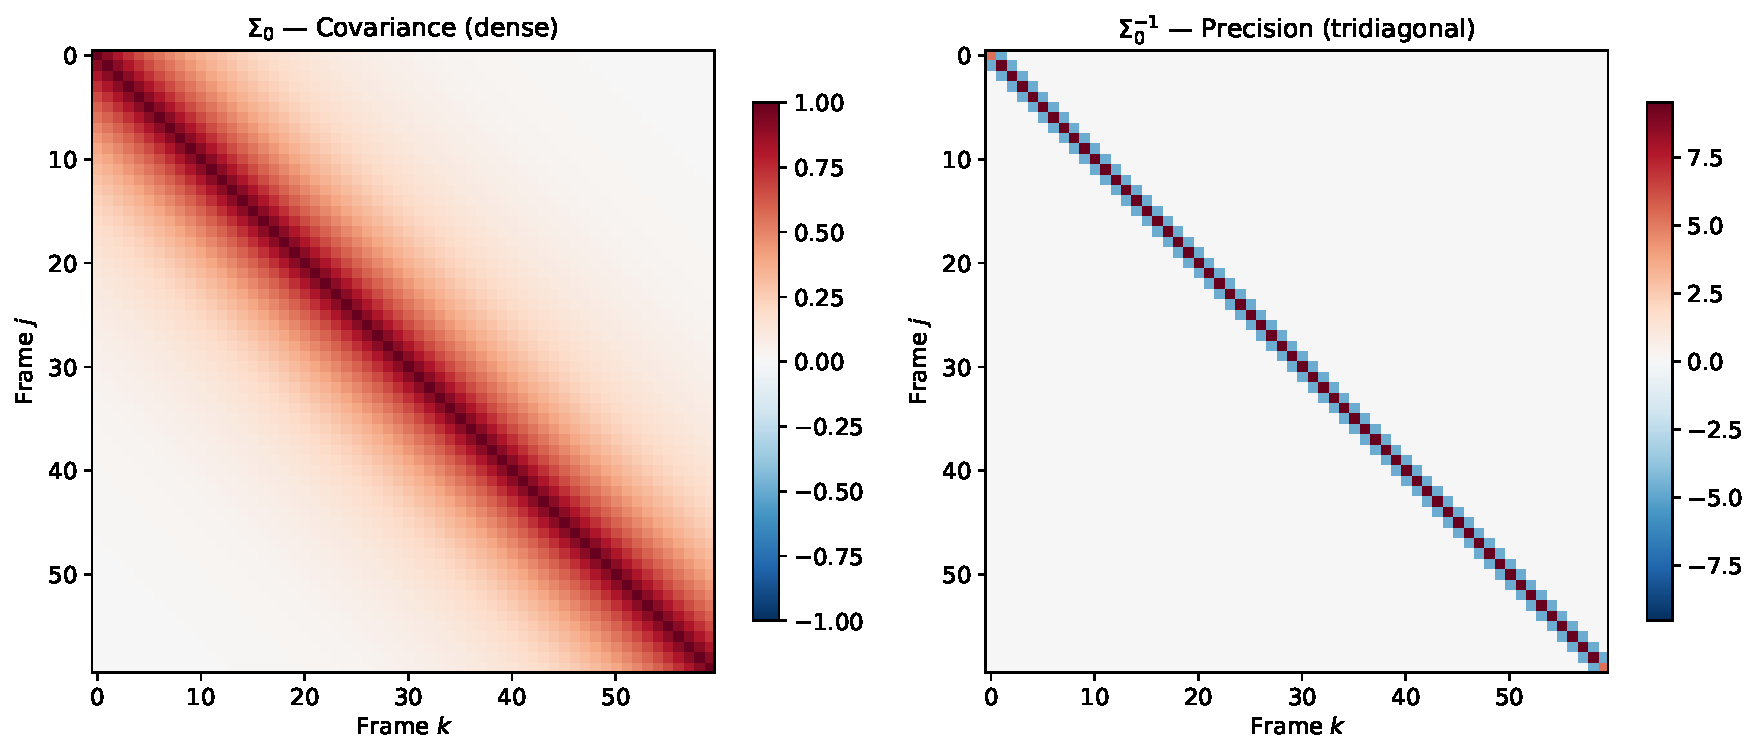
\includegraphics[width=\textwidth]{figures/fig1_clean.pdf}
  \caption{$\Sigma_0$ (left) vs.\ $\Sigma_0^{-1}$ (right) for 60 frames with $\alpha = 0.9$.  The covariance encodes total (marginal) correlations and is dense.  The precision encodes direct (conditional) couplings and is tridiagonal: the Markov property in matrix form.}
  \label{fig:clean}
\end{figure}


% ═════════════════════════════════════════════════════════════════════
\section{$\Sigma_t^{-1}$: Four Representations}
\label{sec:inversion}
% ═════════════════════════════════════════════════════════════════════

We now invert $\Sigma_t = e^{-2t}\Sigma_0 + \Dt I$ in four different ways, each revealing a different aspect of the answer.

\medskip
\textbf{Notation.}
Define the \emph{signal-to-noise ratio} $\gamma_t = e^{-2t}/\Dt$, which goes from $\infty$ (at $t=0$, pure signal) through $1$ (at $t = \frac{1}{2}\ln 2 \approx 0.347$, equal parts) to $0$ (at $t \to \infty$, pure noise).

\begin{keybox}[The four formulas]
\begin{align}
  \Sigma_t^{-1} &= \frac{1}{\Dt}\bigl(I + \gamma_t\,\Sigma_0\bigr)^{-1} \label{eq:factored} \tag{F1: Factored}\\[6pt]
  &= \Sigma_0^{-1}\bigl(e^{-2t}I + \Dt\,\Sigma_0^{-1}\bigr)^{-1} \label{eq:mezard} \tag{F2: M\'ezard}\\[6pt]
  &= \frac{1}{\Dt}I - \frac{e^{-2t}}{\Dt^2}\,\Sigma_0\bigl(\Sigma_0^{-1} + \gamma_t I\bigr)^{-1} \label{eq:woodbury} \tag{F3: Woodbury}\\[6pt]
  &= U\,\diag\!\Bigl(\frac{1}{e^{-2t}d_m + \Dt}\Bigr)_{m=0}^K\,U^\top \label{eq:spectral} \tag{F4: Spectral}
\end{align}
where $\Sigma_0 = U\diag(d_0,\dots,d_K)U^\top$ is the eigendecomposition of $\Sigma_0$.
\end{keybox}

Let us derive and interpret each one.

\subsection{F1: Factored form --- what controls the overall scale}

\begin{proof}
Factor $\Dt$ from $\Sigma_t$:
$\Sigma_t = \Dt\bigl(I + (e^{-2t}/\Dt)\Sigma_0\bigr) = \Dt\bigl(I + \gamma_t\Sigma_0\bigr)$.
Invert: $\Sigma_t^{-1} = (1/\Dt)(I + \gamma_t\Sigma_0)^{-1}$.
\end{proof}

\begin{intbox}[What F1 tells us]
The prefactor $1/\Dt$ sets the overall scale: as $t \to \infty$, $\Dt \to 1$ and the scale is $O(1)$.
The ``shape'' of $\Sigma_t^{-1}$ is controlled by $(I + \gamma_t\Sigma_0)^{-1}$.

When $\gamma_t \gg 1$ (small $t$, strong signal): the $\gamma_t\Sigma_0$ term dominates, so $(I + \gamma_t\Sigma_0)^{-1} \approx (\gamma_t\Sigma_0)^{-1} = \Sigma_0^{-1}/\gamma_t$, and $\Sigma_t^{-1} \approx \Sigma_0^{-1}/e^{-2t}$---tridiagonal.

When $\gamma_t \ll 1$ (large $t$, strong noise): the $I$ term dominates, so $(I + \gamma_t\Sigma_0)^{-1} \approx I$, and $\Sigma_t^{-1} \approx I/\Dt$---diagonal, fully decoupled.

The parameter $\gamma_t$ is the ``dial'' that interpolates between Markov structure and isotropy.
\end{intbox}


\subsection{F2: M\'ezard's form --- why the zeros fill in}

\begin{proof}
Left-multiply $\Sigma_t = e^{-2t}\Sigma_0 + \Dt I$ by $\Sigma_0^{-1}$:
$\Sigma_0^{-1}\Sigma_t = e^{-2t}I + \Dt\Sigma_0^{-1}$.
Therefore $\Sigma_t^{-1} = (\Sigma_0^{-1}\Sigma_t)^{-1}\Sigma_0^{-1} = (e^{-2t}I + \Dt\Sigma_0^{-1})^{-1}\Sigma_0^{-1}$.
\end{proof}

\begin{intbox}[What F2 tells us]
This formula writes $\Sigma_t^{-1}$ as a product of two matrices: $\Sigma_0^{-1}$ (tridiagonal) and $(e^{-2t}I + \Dt\Sigma_0^{-1})^{-1}$.
The matrix $B = e^{-2t}I + \Dt\Sigma_0^{-1}$ is tridiagonal (a diagonal shift of a tridiagonal matrix is still tridiagonal).
But---and this is the crux---\textbf{the inverse of a tridiagonal matrix is generically full}.

Why?
Each entry of $B^{-1}$ involves cofactors of all rows and columns of $B$ (via the adjugate formula $(B^{-1})_{jk} = (-1)^{j+k}M_{kj}/\det B$).
No cancellation makes these entries vanish.
Alternatively: the eigendecomposition $B^{-1} = \sum_m (1/\beta_m)\mathbf{u}_m\mathbf{u}_m^\top$ sums over all eigenvectors, and since the eigenvectors $\mathbf{u}_m(k)$ are nonzero at every position $k$, every entry $(B^{-1})_{jk}$ receives contributions from every mode.

The product of a tridiagonal matrix ($\Sigma_0^{-1}$) with a full matrix ($B^{-1}$) is full.
This is the mechanism by which diffusion noise fills in the Markov zeros.
\end{intbox}


\subsection{F3: Woodbury form --- the noise floor plus a signal correction}

The Woodbury identity $(A + UCV)^{-1} = A^{-1} - A^{-1}U(C^{-1} + VA^{-1}U)^{-1}VA^{-1}$ with $A = \Dt I$, $C = e^{-2t}\Sigma_0$, $U = V = I$ gives F3.

\begin{intbox}[What F3 tells us]
$\Sigma_t^{-1}$ splits into two pieces: a ``noise floor'' $I/\Dt$ (diagonal, no coupling) minus a ``signal correction'' that carries all the inter-frame structure.
At large $t$, the correction vanishes and the noise floor is all that remains.

Moreover, if $\gamma_t < 1/\|\Sigma_0\|$ (which holds at large enough $t$), we can expand $(I + \gamma_t\Sigma_0)^{-1}$ as a Neumann series:
\begin{equation}\label{eq:neumann}
  \Sigma_t^{-1} = \frac{1}{\Dt}\sum_{n=0}^{\infty}(-\gamma_t)^n\Sigma_0^n.
\end{equation}
This is a \textbf{band-by-band expansion}: $\Sigma_0^0 = I$ (diagonal), $\Sigma_0^1$ is tridiagonal, $\Sigma_0^2$ is pentadiagonal (bandwidth 2), and $\Sigma_0^n$ has bandwidth $n$.
The series literally builds $\Sigma_t^{-1}$ by adding one more diagonal band at each order.
Figure~\ref{fig:neumann} shows this in action.
\end{intbox}


\subsection{F4: Spectral form --- the definitive formula}

\begin{theorem}[Spectral decomposition]\label{thm:spectral}
Let $\Sigma_0 = UDU^\top$ be the eigendecomposition, with $U$ orthogonal and $D = \diag(d_0,\dots,d_K)$, $d_0 \geq \cdots \geq d_K > 0$.
Then for all $t \geq 0$:
\begin{equation}\label{eq:spectral}
  \Sigma_t^{-1} = U\,\diag\!\Bigl(\frac{1}{e^{-2t}d_0 + \Dt},\;\dots,\;\frac{1}{e^{-2t}d_K + \Dt}\Bigr)U^\top = \sum_{m=0}^{K}\frac{\mathbf{u}_m\mathbf{u}_m^\top}{e^{-2t}d_m + \Dt}.
\end{equation}
\end{theorem}

\begin{proof}
Since $\Sigma_0 = UDU^\top$ and $I = UU^\top$:
\[
  \Sigma_t = U\bigl(e^{-2t}D + \Dt I\bigr)U^\top.
\]
The matrix in the middle is diagonal with entries $e^{-2t}d_m + \Dt$.
Inverting: $\Sigma_t^{-1} = U\diag(1/(e^{-2t}d_m + \Dt))U^\top$.

The key step: adding $\Dt I$ to $e^{-2t}\Sigma_0$ shifts every eigenvalue by $\Dt$ but \emph{leaves every eigenvector unchanged}, because $I$ has every vector as an eigenvector.
This is why $\Sigma_t$ and $\Sigma_0$ share the same eigenvectors for all $t$.
\end{proof}

\begin{keybox}[The central insight]
The eigenvectors of $\Sigma_t^{-1}$ are the eigenvectors of $\Sigma_0$, independent of $t$.

Only the eigenvalues change: $\lambda_m(t) = e^{-2t}d_m + \Dt$.
As $t$ increases, all eigenvalues converge to 1 (from above for slow modes $d_m > 1$, from below for fast modes $d_m < 1$).
The matrix goes from anisotropic (elongated ellipsoid) to isotropic (sphere).

This shared-eigenvector property is a consequence of \textbf{Gaussianity} (not Markovianity) combined with \textbf{isotropic noise} ($\Dt\cdot I$).
Any Gaussian $P_0$ with any covariance structure would have the same property.
Markovianity determines \emph{which} eigenvectors arise (spatially localised, sine-like modes for the AR(1) chain) and \emph{how} the eigenvalues are distributed.
\end{keybox}


% ═════════════════════════════════════════════════════════════════════
\section{The Eigenbasis: Full Independence}
\label{sec:eigenbasis}
% ═════════════════════════════════════════════════════════════════════

\subsection{Change of basis}

Define rotated variables $\tilde{\mathbf{x}} = U^\top\mathbf{x}$, where $U$ is the eigenvector matrix of $\Sigma_0$.
Since $U$ is orthogonal, this is a rigid rotation---no stretching, no information loss.

\begin{theorem}[Decoupling]\label{thm:decouple}
In the eigenbasis:
\begin{enumerate}[label=(\roman*), nosep]
  \item The score splits into independent scalar components:
  \begin{equation}\label{eq:score-rot}
    \tilde{S}_m(\tilde{\mathbf{x}},t) = -\frac{\tilde{x}_m - \tilde{\mu}_{t,m}}{e^{-2t}d_m + \Dt}.
  \end{equation}
  Each $\tilde{S}_m$ depends only on $\tilde{x}_m$---no coupling between modes.
  \item The noisy distribution factorises: $P_t(\tilde{\mathbf{x}}) = \prod_{m=0}^K\mathcal{N}(\tilde{x}_m;\;\tilde{\mu}_{t,m},\;e^{-2t}d_m + \Dt)$.
  \item The reverse diffusion SDE decouples into $K+1$ independent scalar Ornstein--Uhlenbeck processes.
\end{enumerate}
\end{theorem}

\begin{proof}
For (i): $\tilde{S} = U^\top S(U\tilde{\mathbf{x}},t) = -U^\top\Sigma_t^{-1}U(\tilde{\mathbf{x}}-\tilde{\bm{\mu}}_t)$.
By Theorem~\ref{thm:spectral}, $U^\top\Sigma_t^{-1}U = \diag(1/\lambda_m(t))$, giving~\eqref{eq:score-rot}.

For (ii): $U^\top\Sigma_t U = \diag(\lambda_m(t))$ is diagonal, so the Gaussian factorises.

For (iii): the reverse SDE $d\mathbf{x} = (\mathbf{x} + 2S)\,dt + \sqrt{2}\,d\mathbf{W}$ in the rotated basis uses $\tilde{\mathbf{W}} = U^\top\mathbf{W}$.
Since $U$ is orthogonal and $\mathbf{W}$ has independent components, $\tilde{\mathbf{W}}$ also has independent components (rotating i.i.d.\ Gaussian noise gives i.i.d.\ Gaussian noise---the Gaussian distribution is spherically symmetric).
\end{proof}

\begin{intbox}[What this means in practice]
In the original frame basis, computing the score requires solving a coupled $K\!+\!1$-dimensional system.
In the eigenbasis, it reduces to $K\!+\!1$ independent 1D problems.
Each mode $m$ is a standalone scalar denoiser with its own effective signal-to-noise ratio $\text{SNR}_m(t) = e^{-2t}d_m/\Dt = \gamma_t\,d_m$.

\textbf{Slow modes} (large $d_m$): high SNR, retain signal to large $t$, carry the long-range temporal structure.

\textbf{Fast modes} (small $d_m$): low SNR, overwhelmed by noise early, carry the frame-to-frame fluctuations.

This hierarchy of SNRs is the spectral fingerprint of the AR(1) dynamics on the score.
\end{intbox}


% ═════════════════════════════════════════════════════════════════════
\section{Numerical Study: 60 Frames}
\label{sec:numerical}
% ═════════════════════════════════════════════════════════════════════

We now visualise all results for $K = 59$ (60 frames), $\alpha = 0.9$, $\se = 1-\alpha^2 = 0.19$, $\sinf = 1$.

\subsection{$\Sigma_t^{-1}$ at four diffusion times}

\begin{figure}[H]
  \centering
  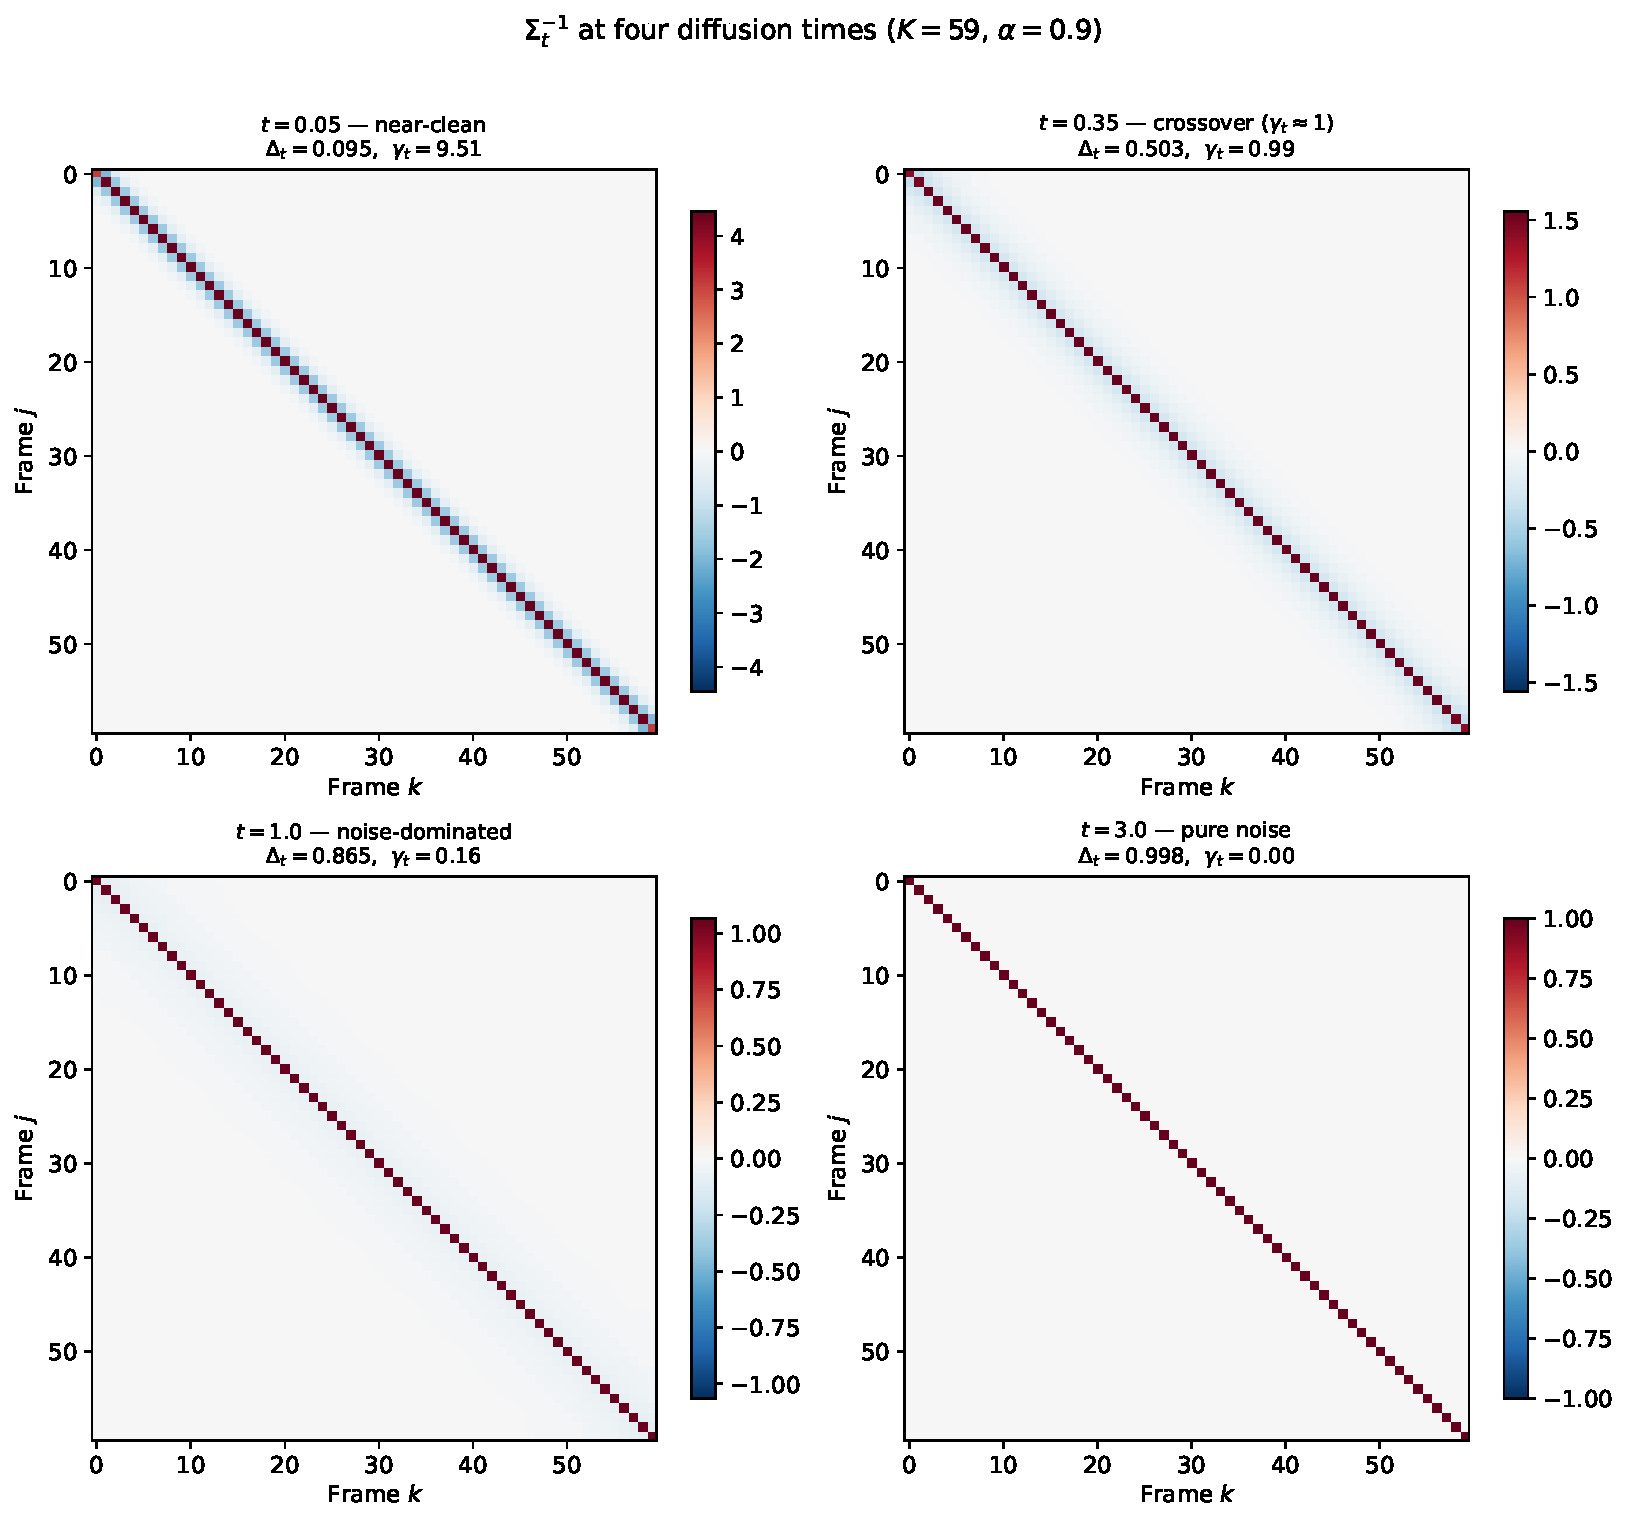
\includegraphics[width=\textwidth]{figures/fig2_prec_t.pdf}
  \caption{$\Sigma_t^{-1}$ at four diffusion times.
  At $t = 0.05$ ($\gamma_t = 10.0$): the tridiagonal structure is visible; the dominant entries are on the three central diagonals.
  At $t = 0.35$ ($\gamma_t \approx 1$, the crossover): the zeros are filled but the tridiagonal band is still the strongest.
  At $t = 1.0$ ($\gamma_t = 0.16$): near-diagonal, with small uniform off-diagonal entries.
  At $t = 3.0$ ($\gamma_t = 0.003$): essentially the identity matrix.}
  \label{fig:prec-t}
\end{figure}

\subsection{How coupling decays with distance}

\begin{figure}[H]
  \centering
  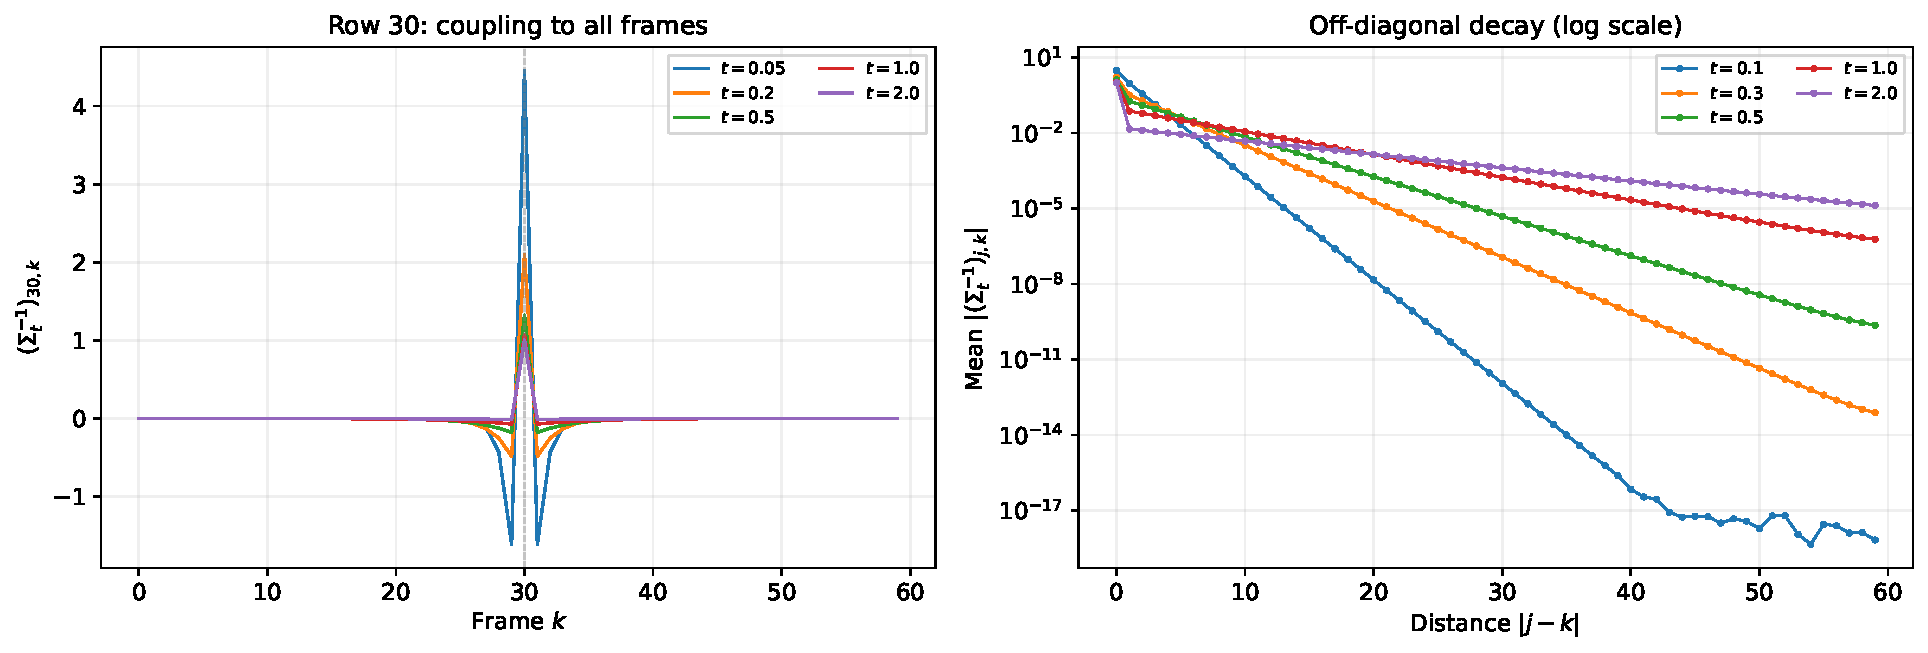
\includegraphics[width=\textwidth]{figures/fig3_coupling.pdf}
  \caption{Left: row~30 of $\Sigma_t^{-1}$ at several diffusion times.  At $t = 0.05$, the coupling is sharply peaked at the nearest neighbours ($k = 29, 31$).  As $t$ grows, the peak broadens and flattens.
  Right: mean $|(\Sigma_t^{-1})_{jk}|$ as a function of distance $|j-k|$ (log scale).  At all $t > 0$ the decay is approximately exponential.  The slope (decay rate) steepens with $t$, because the signal-to-noise ratio drops.}
  \label{fig:coupling}
\end{figure}

\subsection{Tridiagonal weight fraction and condition number}

\begin{figure}[H]
  \centering
  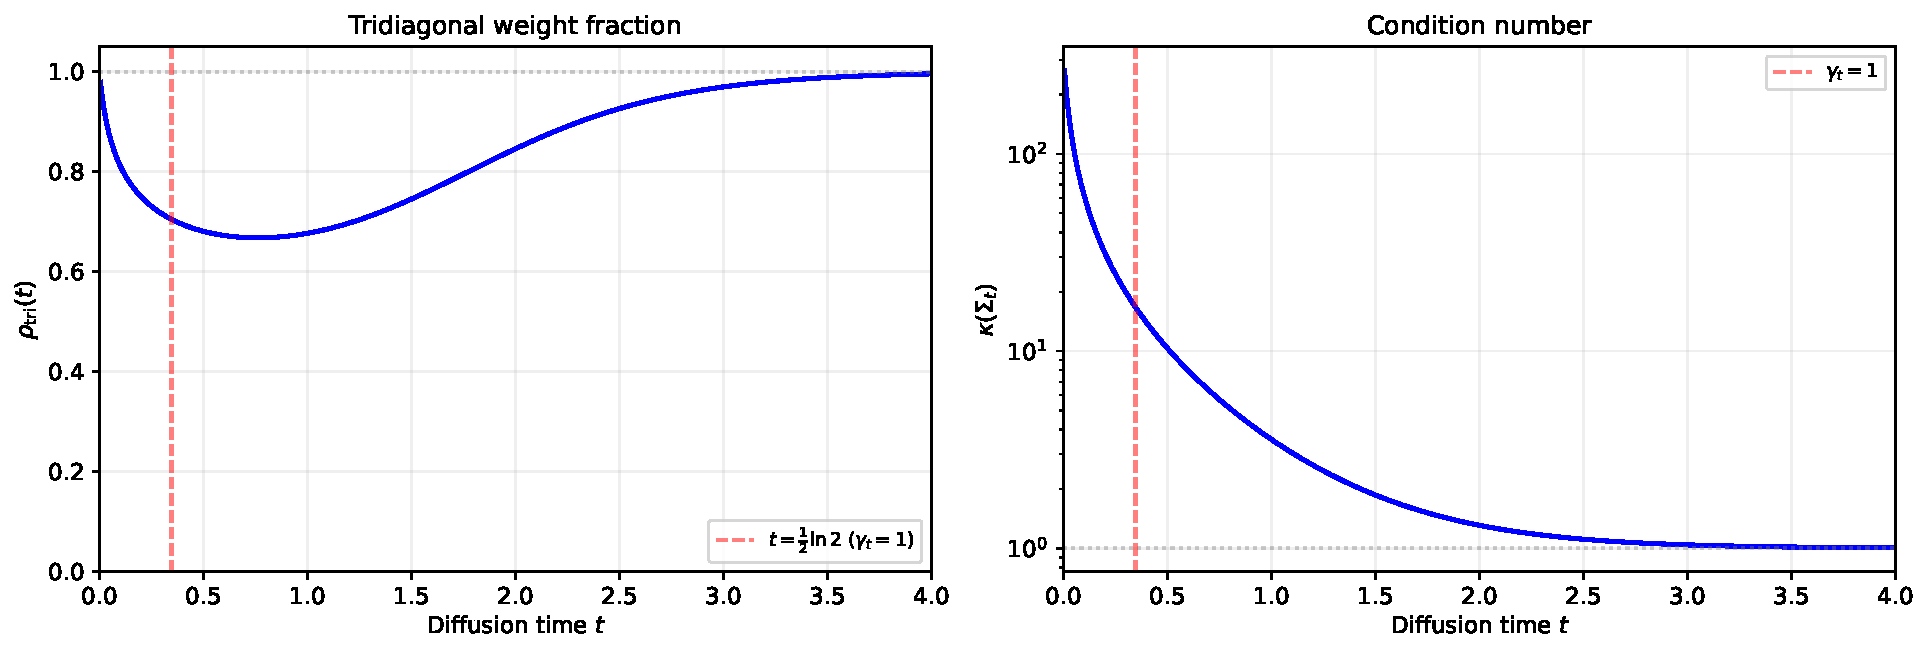
\includegraphics[width=\textwidth]{figures/fig4_diagnostics.pdf}
  \caption{Left: the fraction of $\|\Sigma_t^{-1}\|_1$ (entry-wise) living on the tridiagonal band.  At $t = 0$: 100\%.  The red dashed line marks $\gamma_t = 1$ (crossover), where $\rho_{\mathrm{tri}} \approx 0.6$.
  Right: the condition number $\kappa(\Sigma_t) = \lambda_{\max}/\lambda_{\min}$ drops from $\sim 315$ (anisotropic signal) to $1$ (isotropic noise).}
  \label{fig:diagnostics}
\end{figure}

\subsection{Eigenvalue spectrum and eigenvectors}

\begin{figure}[H]
  \centering
  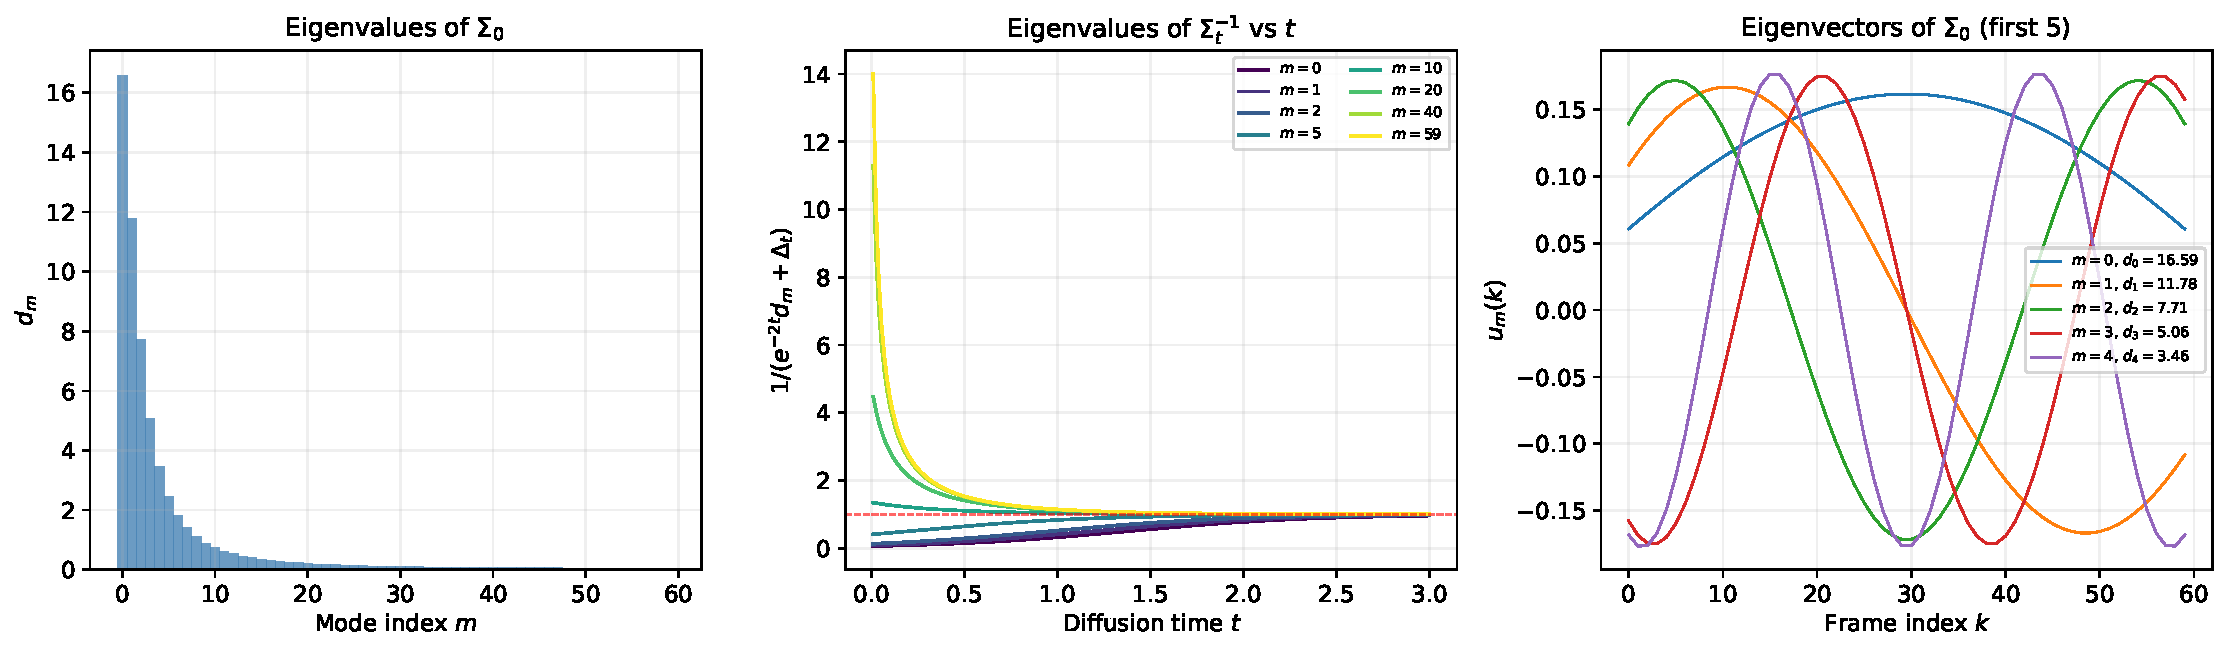
\includegraphics[width=\textwidth]{figures/fig5_spectral.pdf}
  \caption{Left: eigenvalues of $\Sigma_0$.  The slowest mode ($m=0$) has $d_0 \approx 16.6$; the fastest ($m=59$) has $d_{59} \approx 0.053$.  The ratio is $\sim 315$, the condition number.
  Middle: eigenvalues of $\Sigma_t^{-1}$ as functions of $t$ for selected modes.  All converge to $1$.  Slow modes ($m=0$) stay large longer; fast modes ($m=59$) collapse to 1 quickly.
  Right: the first five eigenvectors of $\Sigma_0$.  They are smooth, spatially localised oscillations (approximately sine functions), with mode $m$ having $m$ zero-crossings.  These are the ``Fourier-like'' modes of the AR(1) chain.}
  \label{fig:spectral}
\end{figure}

\subsection{$\Sigma_t^{-1}$ in the eigenbasis: perfect diagonality}

\begin{figure}[H]
  \centering
  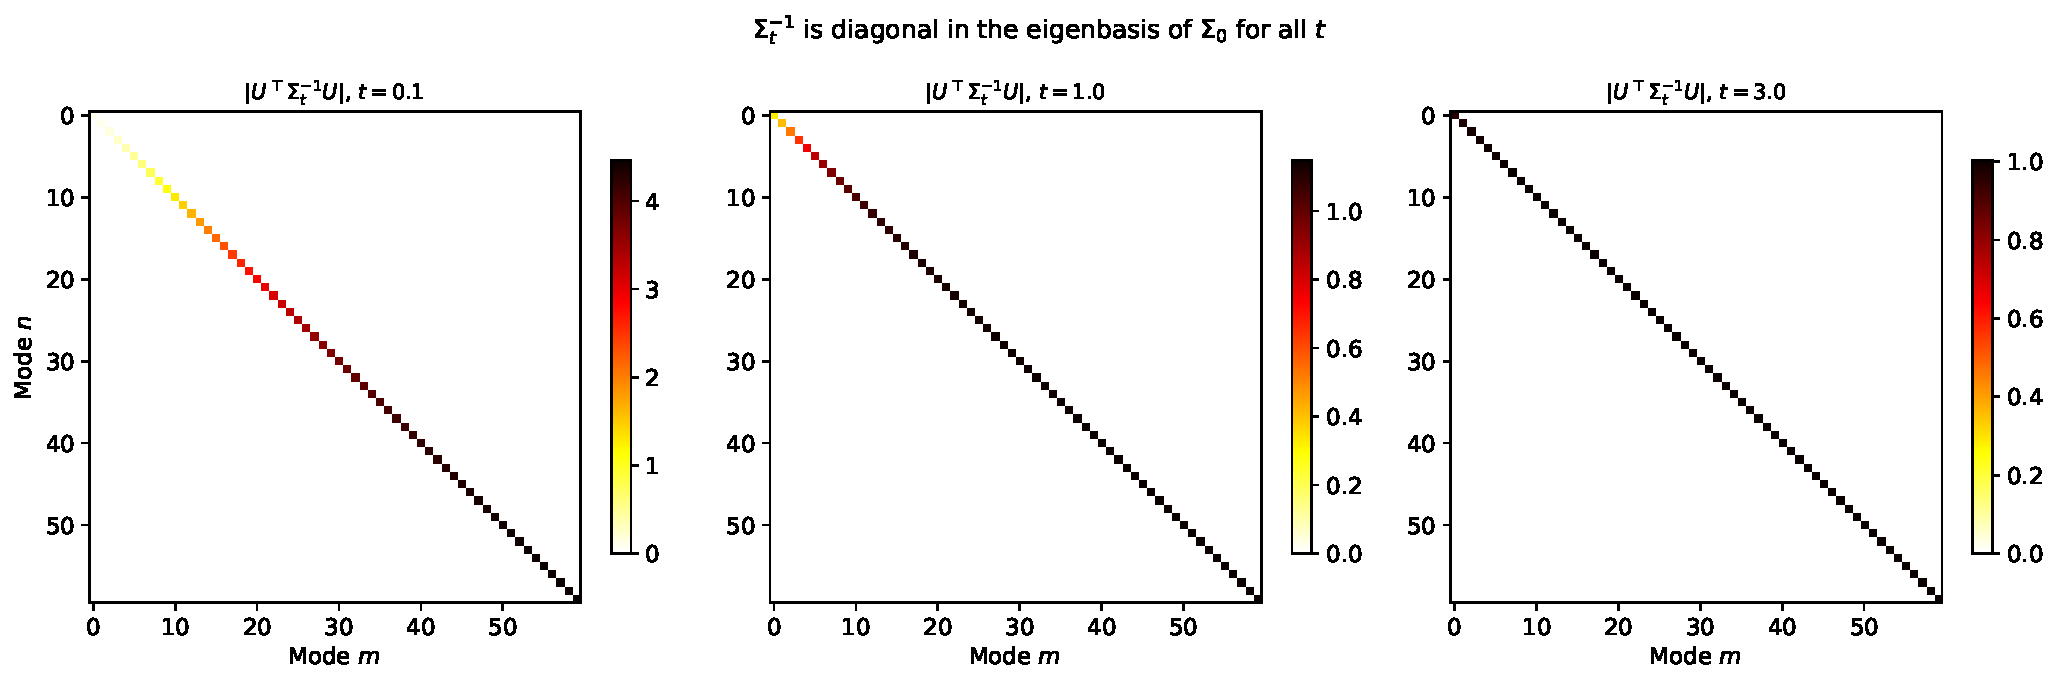
\includegraphics[width=\textwidth]{figures/fig6_eigenbasis.pdf}
  \caption{The matrix $|U^\top\Sigma_t^{-1}U|$ at three diffusion times.  It is exactly diagonal at all $t$, confirming that the eigenvectors of $\Sigma_0$ diagonalise $\Sigma_t^{-1}$ simultaneously for all $t$.  The diagonal entries are $1/(e^{-2t}d_m + \Dt)$.}
  \label{fig:eigenbasis}
\end{figure}

\subsection{The Neumann series: building $\Sigma_t^{-1}$ band by band}

\begin{figure}[H]
  \centering
  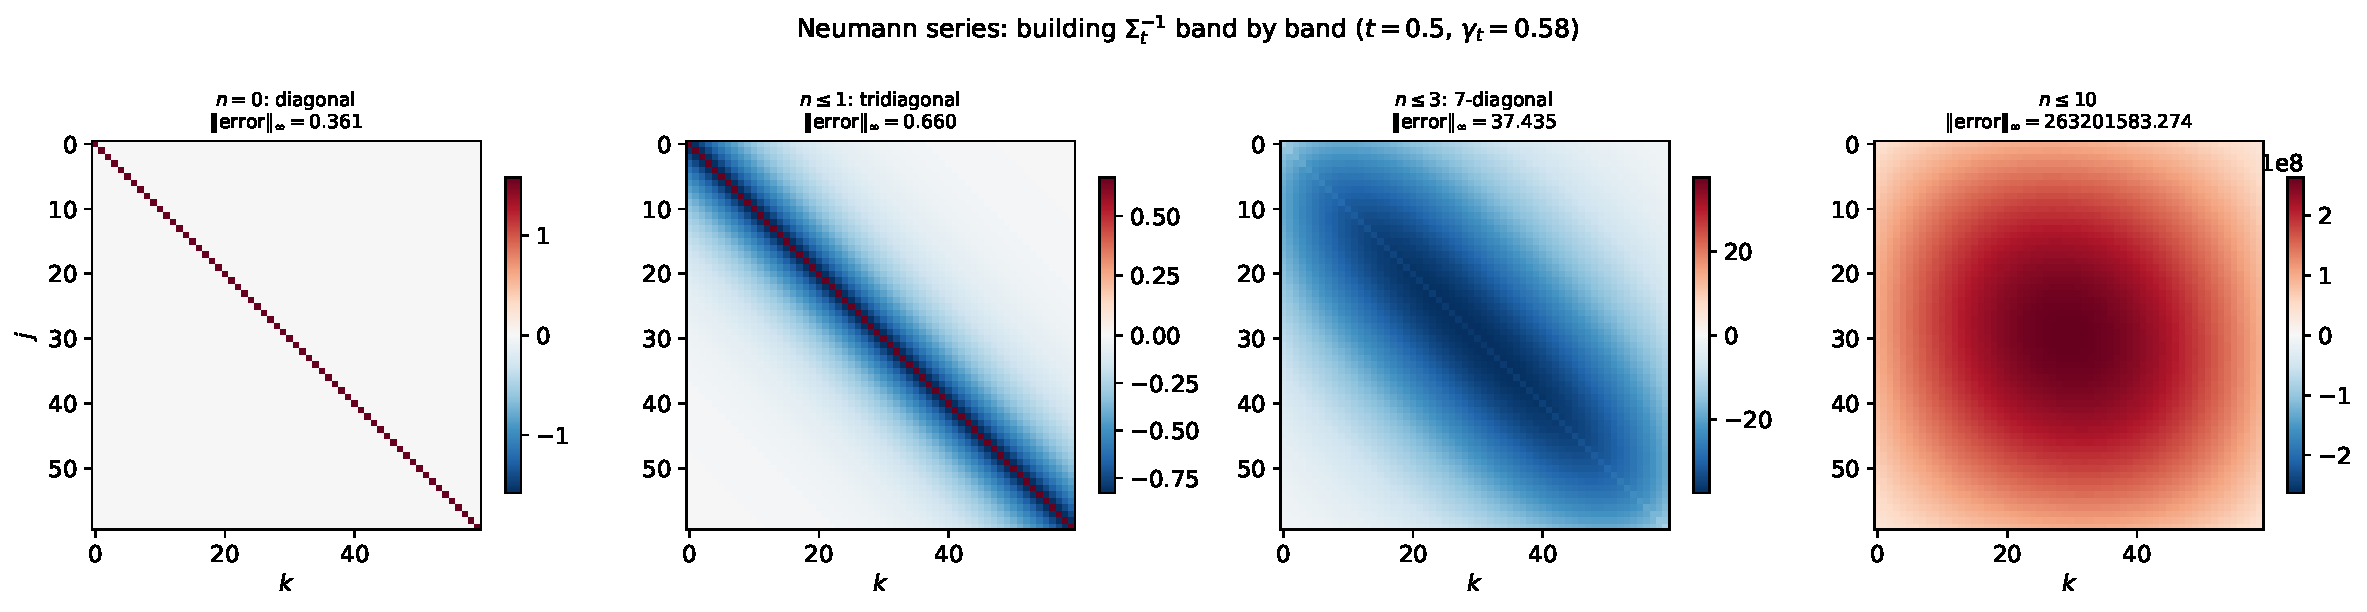
\includegraphics[width=\textwidth]{figures/fig7_neumann.pdf}
  \caption{Partial sums of the Neumann series $\Sigma_t^{-1} = (1/\Dt)\sum_{n=0}^{\infty}(-\gamma_t)^n\Sigma_0^n$ at $t = 0.5$ ($\gamma_t = 0.58$).
  At $n=0$: the diagonal approximation $I/\Dt$.
  At $n\leq 1$: the tridiagonal correction is added.
  At $n\leq 3$: seven diagonals.
  By $n \leq 10$: the error is negligible.  Each order adds one more band of coupling, showing how inter-frame correlations are built up perturbatively from the Markov nearest-neighbour structure.}
  \label{fig:neumann}
\end{figure}


% ═════════════════════════════════════════════════════════════════════
\section{Interpretation: What We Learned}
\label{sec:interpretation}
% ═════════════════════════════════════════════════════════════════════

\subsection{The lifecycle of Markov structure in the score}

As diffusion time $t$ increases from $0$ to $\infty$, the precision matrix $\Sigma_t^{-1}$ undergoes a continuous transformation:
\begin{enumerate}[nosep, leftmargin=2em]
  \item \textbf{$t \approx 0$ (clean signal)}: $\Sigma_t^{-1} \approx e^{2t}\Sigma_0^{-1}$, tridiagonal.  The score couples each frame only to its nearest neighbours.  Full Markov structure.
  \item \textbf{Small $t$ ($\gamma_t \gg 1$)}: the zeros begin to fill in, but the tridiagonal entries remain dominant.  The beyond-tridiagonal entries decay exponentially with distance from the diagonal.  The Markov ``fingerprint'' is strong.
  \item \textbf{Crossover $\gamma_t = 1$ ($t \approx 0.35$)}: signal and noise contribute equally.  The tridiagonal band still carries $\sim 60\%$ of the total weight, but long-range couplings are no longer negligible.
  \item \textbf{Large $t$ ($\gamma_t \ll 1$)}: $\Sigma_t^{-1} \approx I/\Dt$.  Each frame's score depends only on itself.  All inter-frame coupling has been erased.  The score simply pushes each $x_k$ back toward $\mu_{t,k}$.
\end{enumerate}

\subsection{Separating the roles of Gaussianity and Markovianity}

\begin{center}
\renewcommand{\arraystretch}{1.25}
\begin{tabular}{@{}p{7.5cm}ll@{}}
\toprule
\textbf{Property} & \textbf{Requires} \\
\midrule
$\Sigma_0^{-1}$ is tridiagonal (sparse) & Markov \\
$P_t(\mathbf{x})$ is Gaussian; score is linear in $\mathbf{x}$ & Gaussian \\
$\Sigma_t$, $\Sigma_0$ share eigenvectors for all $t$ & Gaussian + isotropic noise\\
Score decouples in eigenbasis & Gaussian + isotropic noise\\
Eigenvectors are sine-like / spatially localised & Markov (tridiagonal $\Sigma_0^{-1}$) \\
$d_m = \se/(1+\alpha^2-2\alpha\cos\theta_m)$ & AR(1) dynamics \\
$|(\Sigma_t^{-1})_{jk}|$ decays with $|j-k|$ & Markov (indirect) \\
\bottomrule
\end{tabular}
\end{center}

\medskip

\textbf{Gaussianity} provides the existence of a fully decoupling eigenbasis.
\textbf{Markovianity} provides the specific structure of that basis (what the eigenvectors look like, what the eigenvalue spectrum is) and is responsible for the spatial localisation of couplings in $\Sigma_t^{-1}$.

If we broke Gaussianity (e.g.\ mixture of Gaussians), the eigenbasis decoupling would fail: the score would become nonlinear in $\mathbf{x}$, and no rotation could make the components independent.
If we broke Markovianity (e.g.\ a Gaussian with long-range correlations), the decoupling would still work, but the eigenvectors and eigenvalues would change.


% ═════════════════════════════════════════════════════════════════════
\section{Looking Ahead}
\label{sec:ahead}
% ═════════════════════════════════════════════════════════════════════

Following the research programme outlined by M\'ezard:

\begin{enumerate}[label=\arabic*., nosep, leftmargin=2em]
  \item \textbf{Enrich $P_0$}: give $P_0$ a non-trivial covariance structure within each frame (multivariate frames with $a_k \in \R^d$), to disentangle intra-frame from inter-frame effects.
  \item \textbf{Break Gaussianity}: replace $P_0$ with a mixture of Gaussians.  The score becomes nonlinear, the eigenbasis trick fails, and the question becomes: does the \emph{Markov} structure (nearest-neighbour dominance) survive in the score even when the Gaussian decoupling does not?
  \item \textbf{Quantify the Markov residual}: define sharper indicators (beyond $\rho_{\mathrm{tri}}$) that measure how much of the score's structure is attributable to Markovianity at each diffusion time.
  \item \textbf{Connect to the Kalman smoother}: the backward pass of the Kalman smoother computes $\langle a_k \rangle_{\mathbf{a}|\mathbf{x}}$ in $O(K)$ time by propagating information from frame $k+1$ to frame $k$.  This propagator is the Markov structure of the score made algorithmic.
\end{enumerate}


% ═════════════════════════════════════════════════════════════════════
\section{Notation}
\label{sec:notation}
% ═════════════════════════════════════════════════════════════════════

\begin{center}
\small
\begin{tabular}{@{}ll@{}}
\toprule
\textbf{Symbol} & \textbf{Meaning} \\
\midrule
$K$ & Number of AR(1) steps; $K+1$ frames total \\
$t \geq 0$ & Diffusion time \\
$\alpha \in (-1,1)$ & AR(1) contraction coefficient \\
$\se$ & Innovation variance; $\sinf = \se/(1-\alpha^2)$ stationary variance \\
$\Dt = 1 - e^{-2t}$ & OU noise variance \\
$\gamma_t = e^{-2t}/\Dt$ & Signal-to-noise ratio \\
$\Sigma_0$, $\Sigma_t = e^{-2t}\Sigma_0 + \Dt I$ & Clean / noisy covariance \\
$d_m$, $\mathbf{u}_m$, $U$ & Eigenvalues, eigenvectors, eigenvector matrix of $\Sigma_0$ \\
$\lambda_m(t) = e^{-2t}d_m + \Dt$ & Eigenvalue of $\Sigma_t$ \\
$\tilde{\mathbf{x}} = U^\top\mathbf{x}$ & Trajectory in the eigenbasis \\
$S(\mathbf{x},t) = -\Sigma_t^{-1}(\mathbf{x}-\bm{\mu}_t)$ & Joint score \\
$\rho_{\mathrm{tri}}(t)$ & Tridiagonal weight fraction of $\Sigma_t^{-1}$ \\
\bottomrule
\end{tabular}
\end{center}

\end{document}
